\addtocontents{toc}{\protect\setcounter{tocdepth}{3}}

\section{Benchmarks}
\label{sec:benchmarks}

Agentic reasoning has been evaluated through a rapidly growing set of benchmarks, but existing suites often differ in what they treat as the core capability, such as tool invocation accuracy, memory retention under long contexts, or coordination quality in multi-agent settings. To provide a coherent view, we organize benchmarks from two complementary perspectives. We first summarize benchmarks that isolate core mechanisms of agentic reasoning, which helps pinpoint where systems succeed or fail at the capability level. We then review application-level benchmarks that evaluate end-to-end agent behavior in realistic domains, capturing the combined effects of perception, planning, tool use, memory, and coordination.

\subsection{Core Mechanisms of Agentic Reasoning}

We begin with benchmarks that target mechanism-level capabilities, aiming to evaluate agentic reasoning in a more controlled and interpretable manner. Concretely, these benchmarks decompose agentic behavior into a small set of recurring primitives, including tool use, search, memory and planning, and multi-agent coordination. Such mechanism-centric evaluations make it easier to attribute performance changes to specific components, and they complement end-to-end benchmarks that may conflate multiple sources of errors.


\begin{figure}
    \centering
    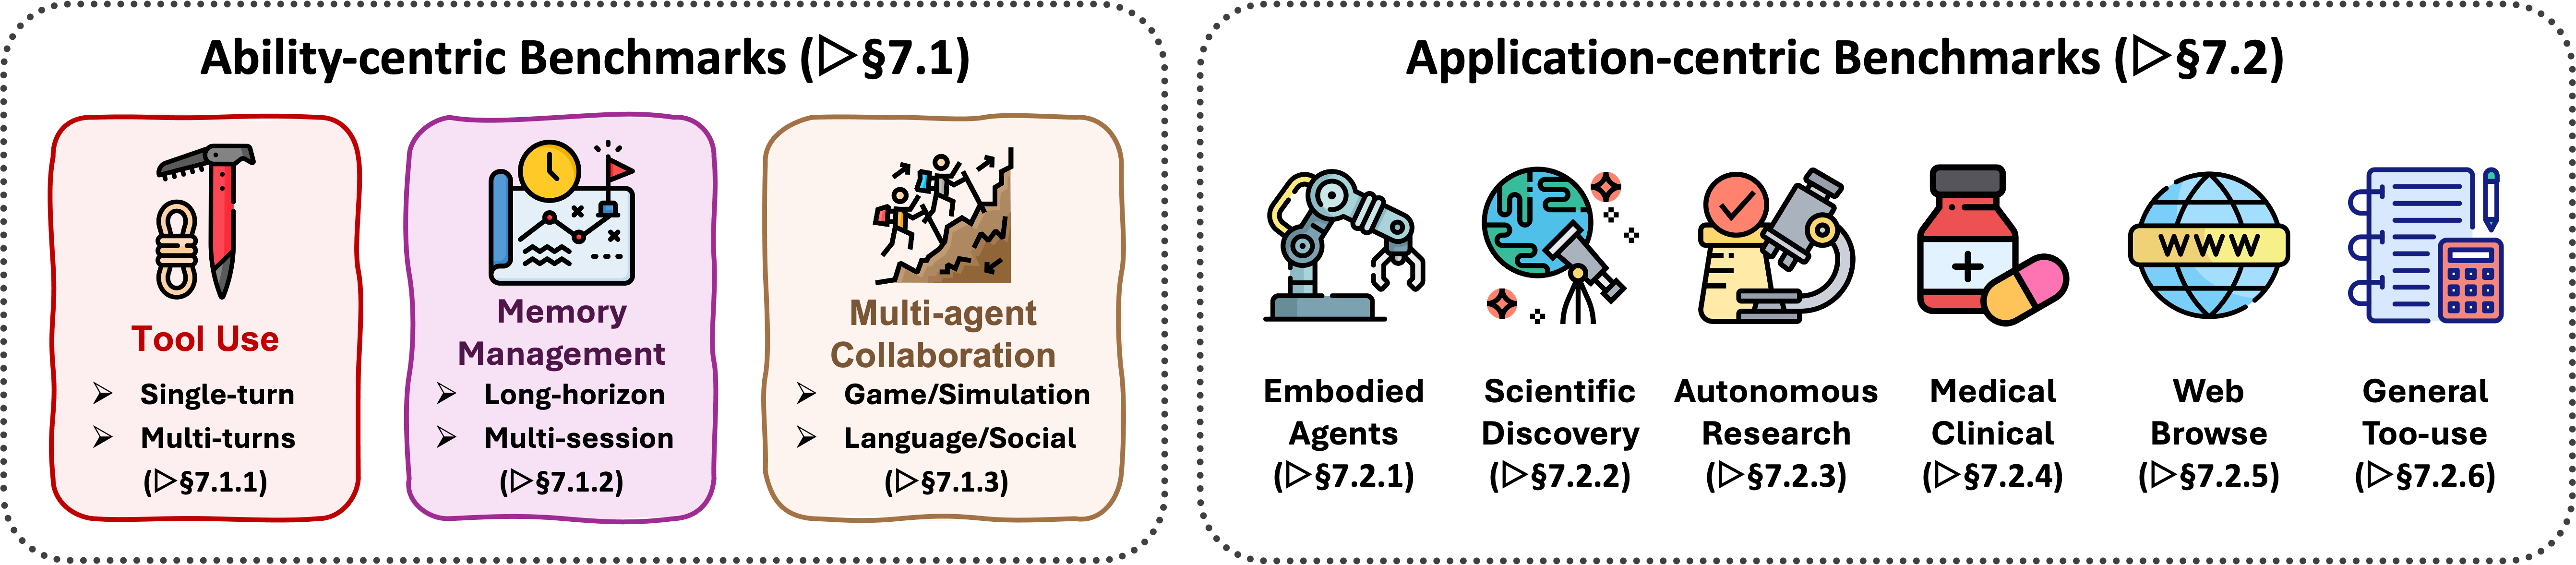
\includegraphics[width=\linewidth]{arxiv/figs/benchmark.png}
    \caption{An overview of the benchmarks on agentic reasoning.}
    \label{fig:benchmark}
\end{figure}


\subsubsection{Tool Use}
Evaluating tool-using models remains an open challenge due to the diversity of tasks, tools, and usage scenarios involved \cite{DBLP:journals/csur/QinHLCDCZZHXHFSWQTZLSXZ25}. The key difficulties arise from the wide range of available tools, varying levels of scenario complexity, and the prevalence requirements specifically for the task domain.

\paragraph{Single-Turn Tool Use.}
While agentic reasoning often focuses on multi-turn or long-horizon interactions, single-turn tool use remains a foundational capability for evaluating LLMs' basic tool invocation skills. ToolQA \cite{DBLP:conf/nips/ZhuangYWSZ23} constructs a dataset of 1,530 dialogues involving 13 specialized tools, designed to assess LLMs' ability to interface with external knowledge sources in a question-answering context. APIBench~\cite{patil2024gorilla} introduces a large-scale benchmark grounded in real-world APIs from HuggingFace, TorchHub, and TensorHub, comprising 1,645 unique APIs and 16,450 instruction–API pairs. It is used to train and evaluate Gorilla, an LLM capable of invoking a broad range of APIs, emphasizing generalization across diverse tool interfaces. ToolLLM-ToolBench~\cite{DBLP:conf/iclr/QinLYZYLLCTQZHT24} curates 16,464 real-world APIs across 49 categories from the RapidAPI Hub, and uses ChatGPT to generate diverse, instruction-style prompts for these APIs. The benchmark is used to train ToolLLaMA, a model that demonstrates strong tool-use capabilities and exhibits promising generalization to unseen APIs. MetaTool \cite{DBLP:conf/iclr/HuangSLFWZ000G024} introduces the TOOLE dataset, containing over 20,000 entries and a benchmark comprising approximately 200 tools across diverse scenarios, including software engineering, finance, and art design. It splits tool selection tasks to tool selection with similar choices, tool selection in specific scenarios , tool selection with possible reliability issues, and multi-tool selection. T-Eval \cite{DBLP:conf/acl/ChenDZLLZZZLCZ24} decomposes tool utilization into a series of sub-processes: instruction following, planning, reasoning, retrieval, understanding, and review, and evaluates each step individually to provide a fine-grained assessment of tool-use capabilities. The benchmark includes a total of 23,305 test cases spanning 15 different tools. GTA (General Tool Agents)~\cite{jize2024gta} targets realistic tool-use scenarios by emphasizing real user queries, real-world deployed tools, and multimodal inputs. It introduces 229 challenging tasks grounded in practical applications, spanning 14 tools across diverse domains. ToolRet \cite{DBLP:journals/corr/abs-2503-01763} focuses specifically on the task of tool retrieval, introducing a heterogeneous benchmark consisting of 7.6K diverse retrieval tasks and a corpus of 43K tools.


\paragraph{Multi-Turn Tool Use.}
Multi-turn tool use offers a more realistic simulation of real-world applications, where agents autonomously select and sequence tools to solve complex tasks. ToolAlpaca \cite{DBLP:journals/corr/abs-2306-05301} is one of the earliest efforts in this direction, using multi-agent simulations to generate 3,938 tool-use instances from over 400 real-world APIs across 50 distinct categories. SambaNova-ToolBench \cite{DBLP:journals/corr/abs-2305-16504} introduces a benchmark centered on software tool manipulation for real-world tasks, with varying levels of API complexity to test agent capabilities. API-Bank \cite{DBLP:conf/emnlp/LiZ000YLHL23} provides a dataset of 1,888 tool-use dialogues from 2,138 APIs, along with a runnable evaluation system containing 73 APIs and 314 tool-use test cases.  UltraTool \cite{DBLP:conf/acl/HuangZLZGLHZWSJ24} evaluates tool-use capabilities across six dimensions: planning awareness, planning ability, creation, tool-use awareness, tool selection, and tool usage. The benchmark spans 22 domains, includes 2,032 tools, and provides 5,824 evaluation samples. ToolFlow distinguishes itself from prior benchmarks by emphasizing long-term planning. It features 224 expert-curated tasks involving 107 real-world tools, highlighting challenges in goal decomposition and multi-step decision-making. More recently, MTU-Bench \cite{DBLP:conf/iclr/WangWWLSPDZWPZG25} presents a multi-granularity benchmark for multi-turn, multi-tool scenarios, and releases MTU-Instruct, a large-scale instruction dataset containing 54,798 dialogues involving 136 tools. m \& m's introduces a benchmark with over 4,000 multi-step, multimodal tasks involving 33 tools, including multimodal models, public APIs, and image processing modules. It also provides a high-quality subset of 1,565 task plans that are human-verified and executable end-to-end.

\subsubsection{Search}

To systematically assess an agent’s ability to acquire information through interaction, recent benchmarks cast search as a sequential reasoning problem and can be broadly categorized into unimodal and multimodal settings, differing in the nature of evidence sources, interaction spaces, and grounding requirements.

\paragraph{Unimodal Search.} Recent benchmarks for single-modal agentic search increasingly frame information seeking as a sequential, decision-driven process, emphasizing planning, interaction, and evidence synthesis. For example, WebWalker~\cite{wu2025webwalker} emphasizes structured website traversal, explicitly modeling search as coordinated horizontal exploration and vertical drilling across interconnected pages. To reflect realistic open-world information seeking, InfoDeepSeek~\cite{xi2025infodeepseek} introduces a dynamic Web setting with verifiable yet non-curated answers, highlighting robustness to noise and distributional shift. Several benchmarks scale search along temporal and informational dimensions: Mind2Web 2~\cite{gou2025mind2web2} focuses on long-horizon browsing and citation-grounded synthesis, whereas RAVine~\cite{xu2025ravine} augments answer quality with process-level efficiency and interaction fidelity. Complementarily, WideSearch~\cite{wong2025widesearch} and DeepWideSearch~\cite{lan2025deepwidesearch} distinguish between breadth-oriented large-scale fact aggregation and depth-oriented multi-hop reasoning, revealing the difficulty of jointly optimizing coverage and reasoning coherence. Domain-specific benchmarks further stress reliability under strict correctness constraints: MedBrowseComp~\cite{chen2025medbrowsecomp} targets clinical decision support by requiring agents to integrate heterogeneous and potentially conflicting medical evidence, while FinAgentBench~\cite{choi2025finagentbench} evaluates retrieval-centric reasoning in financial analysis through document-type selection and fine-grained passage localization. Finally, LocalSearchBench~\cite{he2025localsearchbench} grounds agentic search in real-world local services, evaluating multi-constraint, multi-entity reasoning over large structured databases. Collectively, these benchmarks redefine agentic search evaluation around planning depth, interaction quality, evidence integration, and real-world fidelity, providing a more holistic assessment of search-centric reasoning in language-based agents.

\paragraph{Multimodal Search.} Recent benchmarks on multimodal agentic search move beyond static multimodal question answering to systematically evaluate an agent’s ability to actively retrieve, browse, and reason over heterogeneous information sources under realistic constraints. Benchmarks such as MMSearch~\cite{jiang2024mmsearch} and its extension MMSearch-Plus~\cite{tao2025mmsearch} frame multimodal search as an end-to-end process, where agents must interpret multimodal queries and synthesize answers by jointly leveraging textual and visual evidence, explicitly modeling different input–output modality configurations. Complementing this setting, MM-BrowseComp~\cite{li2025mm} adapts the “hard-to-find, easy-to-verify” paradigm to multimodal web environments, enforcing mandatory image dependence to prevent text-only shortcuts and to stress-test multimodal evidence grounding during open-web browsing. BEARCUBS~\cite{song2025bearcubs} further emphasizes computer-using agents in live web scenarios, requiring explicit interaction trajectories and multimodal manipulation (e.g., videos or 3D navigation), thereby evaluating not only retrieval accuracy but also procedural competence. Moving into domain-specific and tool-augmented regimes, PaperArena~\cite{wang2025paperarena} evaluates multimodal agentic search in scientific workflows, where agents must coordinate PDF parsing, figure understanding, database queries, and web search to answer research-level questions. Finally, Video-BrowseComp~\cite{liang2025video} and VideoDR~\cite{liu2026videodr} extend agentic search to video-centric settings, requiring agents to extract visual-temporal cues from videos and iteratively validate hypotheses via open-web evidence, with carefully designed constraints to ensure dual dependence on video and external retrieval. Together, these benchmarks delineate a clear evolution toward evaluating multimodal agents as interactive researchers, highlighting planning, tool use, and multimodal evidence integration as first-class capabilities in agentic search.


\subsubsection{Memory and Planning}

A distinctive advantage of agents lies in their ability to leverage memory to achieve accurate long-term performance and strong reasoning capabilities. This ability can be assessed from two complementary perspectives. The first concerns memory management, which reflects how effectively an agent integrates, organizes, and retrieves long-term memories. The second concerns memory utilization, which captures how well an agent exploits historical information to support planning and informed feedback. In this section, we separately discuss benchmarks from these two aspects.

From the perspective of memory management, existing benchmarks can be broadly categorized into \textit{Long-Horizon Episodic Memory} and \textit{Multi-session Recall}, depending on whether the textual context consists of a single continuous long-form input or multiple discontinuous conversational sessions.

\paragraph{Long-Horizon Episodic Memory.}
This category targets single-episode tasks with partial observability and delayed rewards, requiring agents to store and retrieve information over extended time spans. Benchmarks in this space evaluate memory retention, retrieval, and reasoning across long contexts. PerLTQA \cite{du2024perltqa} simulates personalized dialogue, where agents answer questions using long-term persona and event memories. It includes 8.5K QA pairs and evaluates memory classification, retrieval ranking, and synthesis fidelity. ELITR-Bench \cite{thonet2024elitr} tests QA on noisy meeting transcripts, where relevant evidence may appear far earlier than the query. Models are scored via GPT-4 across various ASR noise levels and dialogue settings. In the meanwhile, Multi-IF \cite{he2024multi} and MultiChallenge \cite{sirdeshmukh2025multichallenge} focus on multi-turn instruction following. Multi-IF \cite{he2024multi} spans 4.5K tri-turn conversations in 8 languages, with evaluation based on strict and relaxed instruction accuracy. MultiChallenge \cite{sirdeshmukh2025multichallenge} tests four memory-intensive phenomena: retention, inference, editing, and coherence, using 273 curated dialogues with binary pass/fail evaluation. TurnBench-MS \cite{zhang2025turnbench} evaluates multi-step reasoning across 540 symbolic logic games, tracking win rate, round-level accuracy, and verifier usage. StoryBench \cite{wan2025storybench} casts memory as decision-making in interactive narratives, where agents must remember prior choices to progress. It assesses decision accuracy, retry counts, and runtime efficiency. MemBench \cite{tan2025membench} tests factual and reflective memory across 60K episodes in participatory and observational settings, with metrics for accuracy, recall, capacity, and retrieval speed. MMRC~\cite{xue2025mmrc} develops a multimodal memory benchmark focused on single-round multimodal conversations. Together, these benchmarks emphasize structured memory demands, with metrics capturing not just task success but also memory precision, synthesis quality, and robustness under long-context stress.

\paragraph{Multi-session Recall.}
Multi-session Recall focuses on multi-episode tasks where agents must retain and integrate knowledge across separate sessions, supporting lifelong adaptation and mitigating catastrophic forgetting. A range of recent benchmarks systematically probe this capability under realistic, long-term interaction scenarios. LOCOMO \cite{maharana2024evaluating} evaluates LLM agents on sustained conversational memory across 19-session dialogues, using tasks such as multi-hop QA, event summarization, and multi-modal response generation. MemSim \cite{zhang2024memsim} introduces a simulator-based framework with over 2,900 synthetic trajectories in daily life domains, assessing fact retention across sessions via accuracy, diversity, and rationality scores. LONGMEMEVAL \cite{wu2024longmemeval} benchmarks assistants on five sub-tasks: information extraction, multi-session reasoning, temporal inference, knowledge updating, and abstention, over dialogue histories spanning up to 1.5M tokens, with GPT-4 judged accuracy and retrieval recall. REALTALK \cite{lee2025realtalk} presents 21-day real human conversations with 17K tokens per dyad, enabling evaluation of memory probing and persona simulation through multi-hop QA and emotional grounding metrics. Furthermore, MemoryAgentBench \cite{hu2025evaluating} unifies diverse memory tasks such as test-time learning, conflict resolution, and long-range understanding across multiple datasets, with task-specific metrics including classification accuracy, partial-match F1, and ROUGE. Mem-Gallery~\cite{bei2026mem} introduces a multimodal long-term memory evaluation benchmark that systematically covers a wide range of memory management and utilization scenarios. Lastly, Evo-Memory \cite{wei2025evo} introduces a benchmark and a unified evaluation protocol for measuring experience reuse in test-time learning. Collectively, these benchmarks underscore the importance of dynamic memory integration across sessions and provide comprehensive evaluations across factual recall, adaptation, and reasoning. 

From the perspective of memory utilization, we provide a detailed discussion of benchmarks that evaluate an agent’s ability to support planning and feedback using historical information.

\paragraph{Planning and Feedback.} Benchmarks targeting planning and feedback primarily assess whether agents can effectively utilize memory to support multi-step planning based on environmental feedback, and maintain coherent internal state over extended interactions. First, ALFWorld~\cite{shridhar2020alfworld} employs interactive environments to evaluate the consistency of multi-step planning, requiring agents to accumulate observations across actions and maintain latent internal states throughout execution. Moreover, formal planning benchmarks such as PlanBench~\cite{valmeekam2023planbench} and ACPBench~\cite{kokel2025acpbench} assess planning capabilities in explicitly defined dynamic environments, testing whether agents can correctly reason about action preconditions, effects, reachability, and overall plan validity. TEXT2WORLD~\cite{hu2025text2world} integrate fragmented textual descriptions into a coherent and executable world model, evaluating the capacity to continuously consolidate historical facts into structured planning representations.
More recent benchmarks place greater emphasis on feedback integration and planning under non-stationary conditions. For example, REALM-Bench~\cite{geng2025realm} introduces dynamic disturbances in real-world manufacturing scenarios, requiring agents to remember prior commitments and replan when underlying assumptions are violated, while TravelPlanner~\cite{xie2024travelplanner} focuses on accurate itinerary construction under constrained and evolving information. Finally, FlowBench~\cite{xiao2024flowbench} and UrbanPlanBench~\cite{zheng2025urbanplanbench} assess planning performance in procedural and domain-specific settings, respectively, where agents must preserve conversational or policy context and apply it consistently across decision steps. Together, these benchmarks go beyond one-shot plan generation and systematically investigate whether agents can leverage historical information to support sustained planning, adaptive feedback integration, and iterative decision revision over time.


\subsubsection{Multi-Agent System}

To evaluate coordination, competition, and decision making beyond isolated reasoning, recent benchmarks situate multi-agent systems in interactive environments. These works broadly span game-based evaluations, simulation-centric real-world scenarios, and language-driven social reasoning tasks.

\paragraph{Game-based reinforcement learning evaluation.}
Game-based reinforcement learning evaluation benchmarks leverage classical and novel gaming environments to systematically compare the performance of multi-agent RL algorithms under cooperative and adversarial settings.
MAgent \citep{zheng2018magent} facilitates massive-scale multi-agent scenarios such as pursuit and resource competition within customizable grid-worlds, evaluating individual cumulative rewards and competitive metrics like resource occupancy rates. Pommerman \citep{resnick2018pommerman} adapts the classic Bomberman game for cooperative and adversarial interactions, quantifying performance through win rates, survival duration, and kill-to-suicide ratios. SMAC \citep{samvelyan2019starcraft} centers on decentralized micromanagement challenges in StarCraft II scenarios, evaluating team success via win rates, average damage output, and formation dispersion.
MineLand \citep{yu2024mineland} utilizes Minecraft as a realistic ecological simulation for large-scale multi-agent coordination, with up to 64 agents cooperating to meet physical needs under partial observability. TeamCraft \citep{long2024teamcraft} also employs Minecraft to benchmark embodied multi-modal agents tasked with interpreting visual, textual, and environmental prompts to collaboratively achieve 55,000 procedurally generated task instances. Melting Pot \citep{leibo2021scalable} assesses agents’ zero-shot generalization capabilities in diverse social dilemma environments, utilizing metrics such as per-capita return, social welfare, and inequality indices. BenchMARL \citep{bettini2024benchmarl} provides standardized algorithm comparisons across multiple scenarios (e.g., SMACv2, VMAS, MPE), measuring convergence rates, final performance, and hyperparameter sensitivity. Finally, Arena \citep{song2020arena} encompasses a comprehensive suite of cooperative and adversarial games across various complexities, evaluating individual returns, collective social welfare, and emergent communication protocols.

\paragraph{Simulation-centric real-world assessment.}
Simulation-centric real-world benchmarks simulate realistic or pseudo-realistic environments, emphasizing scalability, partial observability, and dynamic planning. SMARTS \citep{zhou2020smarts} offers a scalable multi-agent driving platform for real-world traffic scenarios like merges and intersections, with evaluation based on collision rates, task completion, and agent behavior distributions. Nocturne \citep{vinitsky2022nocturne} provides high-throughput, partially observable driving simulations using Waymo trajectories, testing coordination and human-like behavior in tasks such as intersections and roundabouts. MABIM \citep{yang2023versatile} benchmarks multi-echelon inventory management, simulating cooperative and competitive retail dynamics, evaluated via profit metrics across diverse inventory settings. IMP-MARL \citep{leroy2023imp} addresses infrastructure inspection and maintenance scheduling, measuring risk reduction and cost efficiency in large-scale systems. POGEMA \citep{skrynnik2024pogema} focuses on decentralized multi-agent pathfinding in grids, tracking success rate, path efficiency, and large-scale coordination. INTERSECTIONZOO \citep{jayawardana2024intersectionzoo} studies contextual RL for cooperative eco-driving at intersections, using traffic simulations to evaluate emissions and travel-time performance. REALM-Bench \citep{geng2025realm} introduces real-world planning tasks from logistics to disaster relief, with dynamic disruptions, multi-threaded dependencies, and evaluation via planning quality, adaptability, and constraint satisfaction. Together, these benchmarks reflect challenges in scaling, uncertainty, coordination, and dynamic adaptation, offering rigorous testbeds for real-world multi-agent systems.

\paragraph{Language, Communication, and Social Reasoning.}
Benchmarks in Language, Communication, and Social Reasoning explore multi-agent communication protocols, Theory-of-Mind reasoning, game-theoretic interactions, and language-driven coordination. LLM-Coordination \citep{agashe2023llm} examines collaborative reasoning and joint-planning abilities of LLM agents through cooperative gameplay (e.g., Hanabi, Overcooked-AI), measured by holistic scores and fine-grained coordination question accuracy. AVALONBENCH \citep{jonathan2023avalonbench} leverages the social deduction game Avalon to assess role-conditioned language-based reasoning, with datasets of thousands of five-player dialogues and metrics on win-rate, role accuracy, and voting dynamics. Welfare Diplomacy \citep{mukobi2023welfare} extends the classic game Diplomacy to general-sum welfare negotiation, using 50-game datasets to quantify coalition stability and welfare-oriented strategic reasoning. MAgIC \citep{xu2023magic} covers social deduction and classic dilemmas (e.g., Chameleon, Prisoner's Dilemma), employing handcrafted scenario datasets to benchmark reasoning, deception, coordination, and rationality. BattleAgentBench \citep{wang2024battleagentbench} assesses language-based cooperative and competitive dynamics in strategic gameplay environments, scoring navigation accuracy, agent interactions, and exploitability across diverse map datasets. COMMA \citep{ossowski2024comma} evaluates multimodal communicative reasoning through collaborative puzzle-solving tasks involving visual-language coordination, measured by grounding accuracy, privacy compliance, and dialogue effectiveness across thousands of scenarios. IntellAgent \citep{levi2025intellagent} introduces synthetic conversational AI tasks in retail and airline domains, generating extensive policy-constrained dialogue datasets evaluated by conversational success, mistake frequency, and policy adherence. Finally, MultiAgentBench \citep{zhu2025multiagentbench} provides a comprehensive assessment across tasks such as Minecraft building, coding, and bargaining, employing dynamic key-performance indicators and LLM-scored communication quality across various multi-agent topologies and scenarios.

\subsection{Applications of Agentic Reasoning}
\label{sec:app-benchmark}

While mechanism-centric benchmarks help isolate individual capabilities, real-world deployments require these capabilities to work together under realistic constraints, such as partial observability, long-horizon dependencies, and safety-critical decisions. We therefore next review application-level benchmarks that evaluate end-to-end agent performance across representative environments, with tasks that jointly stress perception, reasoning, action execution, and coordination.

In this subsection, we review benchmarks designed to evaluate the application-level performance of agentic reasoning systems across various domains. These benchmarks assess agents' ability to perceive, reason, and act in realistic or high-impact task settings. We organize the discussion into six categories based on the application environment: \textit{Embodied Agents}, \textit{Scientific Discovery Agents}, \textit{Autonomous Research Agents}, \textit{Medical and Clinical Agents}, \textit{Web Agents}, and \textit{Tool-Use Agents}. Each subsubsection introduces representative benchmarks and describes their design motivation, task format, and evaluation metrics.

\subsubsection{Embodied Agents}
Benchmarks under this category evaluate agents that interact with physical or simulated environments, requiring grounding, perception, and action planning. AgentX~\cite{tajamul2025agentx} provides a diverse suite of vision-language embodied tasks in driving and sports, where agents must make decisions using multimodal information from videos. It emphasizes reasoning across scenes with occlusions, temporal gaps, or distractors. BALROG~\cite{davide2024balrog} builds a reinforcement learning-centric framework for benchmarking agentic planning in game environments, focusing on instruction-following, temporal abstraction, and error correction. ALFWorld~\cite{shridhar2020alfworld} links language instructions to object interactions in a text-based 3D environment, evaluating perception-grounded execution. AndroidArena~\cite{mingzhe2024understanding} targets GUI-based mobile tasks, where agents must perform actions like form-filling and app navigation using vision-language understanding. StarDojo~\cite{weihao2025stardojo} leverages the open-ended Stardew Valley game to study social planning and role-based coordination. MindAgent~\cite{ran2023mindagent} and NetPlay~\cite{dominik2024playing} create multiplayer gaming testbeds to benchmark emergent social reasoning and negotiation under uncertainty. OSWorld~\cite{tianbao2024osworld} offers a simulated desktop environment with diverse cross-app productivity tasks, such as opening files, converting formats, and modifying documents. These environments challenge agents to coordinate between perception, planning, and symbolic action in dynamic and often partially observable scenarios.

\subsubsection{Scientific Discovery Agents}
Scientific benchmarks aim to test agents' capabilities in knowledge acquisition, hypothesis generation, and experimental automation. DISCOVERYWORLD~\cite{jansen2024discoveryworld} introduces a virtual lab where agents explore scientific phenomena in biology, chemistry, and physics through simulated tools and instruments. ScienceWorld~\cite{ruoyao2022scienceworld} focuses on elementary science experiments using textual instructions and environment interactions, requiring step-by-step hypothesis testing. ScienceAgentBench~\cite{ziru2024scienceagentbench} builds a benchmark from real-world scientific papers, translating tasks like code implementation, figure generation, and variable extraction into executable subtasks, assessing agents’ ability to automate the research process. The AI Scientist~\cite{chris2024the} simulates a full end-to-end research pipeline, where agents perform literature review, method writing, experiment execution, and peer-review simulation. LAB-Bench~\cite{jon2024labbench} evaluates biology-specific agents on tasks involving genetic sequence reasoning and experiment planning. MLAgentBench~\cite{qian2023mlagentbench} benchmarks agents’ ability to autonomously train, evaluate, and tune machine learning models, offering realistic experimentation workflows. These benchmarks collectively probe open-ended reasoning, long-horizon planning, and scientific grounding in semi-structured data settings.

\subsubsection{Autonomous Research Agents}
This category benchmarks agents designed for long-horizon workflows across general-purpose research, office, or planning tasks. WorkArena~\cite{alexandre2024workarena} and its extension WorkArena++~\cite{leo2024workarena} propose enterprise task benchmarks where agents must complete ticket-based workflows involving retrieval, summarization, and coordination across documents. OfficeBench~\cite{zilong2024officebench} simulates a productivity software suite environment with tasks such as creating meeting memos, modifying spreadsheets, and replying to emails, emphasizing goal decomposition and tool selection. PlanBench~\cite{valmeekam2023planbench} and FlowBench~\cite{xiao2024flowbench} test general workflow planning skills with abstracted task graphs and structured dependencies. ACPBench~\cite{kokel2025acpbench} evaluates agents in assistant–collaborator–planner triads, tracking performance in a hybrid role hierarchy. TRAIL~\cite{darshan2025trail} focuses on multi-agent trace debugging and error attribution~\cite{zhang2024knowledge} in LLM-based systems, providing dense annotations for reasoning chains. CLIN~\cite{bodhisattwa2023clin} introduces lifelong few-shot learning benchmarks where agents adapt to distribution shift and task evolution. Agent-as-a-Judge~\cite{mingchen2024agentasajudge} studies peer-review style evaluation with agents grading reasoning chains and correctness of other agents’ outputs. InfoDeepSeek~\cite{xi2025infodeepseek} measures information-seeking abilities in open-domain QA and synthesis tasks. Together, these benchmarks capture the growing demand for agentic reasoning in complex knowledge workflows that involve abstraction, iteration, and evaluation.

\subsubsection{Medical and Clinical Agents}
These benchmarks test agents’ abilities to reason with clinical knowledge, patient data, and multimodal biomedical sources. AgentClinic~\cite{samuel2024agentclinic} introduces a virtual hospital environment where agents make diagnostic decisions based on patient symptoms and medical imaging. MedAgentBench~\cite{yixing2025medagentbench} combines medical QA, patient simulation, and retrieval tasks in a multi-format benchmark grounded in standardized exams. MedAgentsBench~\cite{xiangru2025medagentsbench} evaluates multi-hop medical reasoning over structured and unstructured data, scoring agents on correctness and evidence alignment. EHRAgent~\cite{wenqi2024ehragent} benchmarks agents working over structured electronic health record (EHR) tables and clinical notes to complete tasks like diagnosis code prediction and medication reasoning. MedBrowseComp~\cite{chen2025medbrowsecomp} focuses on browsing-based medical QA, where agents must retrieve and verify information across web pages. ACC~\cite{thakrar2025architectingclinicalcollaborationmultiagent} explores trustworthy medical agents with retrieval, hallucination detection, and citation-based support evaluation. MedAgents~\cite{xiangru2023medagents} uses a collaborative multi-agent dialogue setup to simulate patient–doctor–nurse interactions, scoring fluency and factual accuracy. GuardAgent~\cite{zhen2024guardagent} proposes a clinical privacy safeguard agent with structured risk detection benchmarks on EHR and website forms. These datasets emphasize correctness, trustworthiness, and safety in real-world clinical deployment contexts.

\subsubsection{Web Agents}
Web agents operate in realistic browsing environments and are benchmarked on their ability to parse layouts, execute actions, and handle dynamic content. WebArena~\cite{shuyan2023webarena} introduces a browser-based benchmark suite containing 90+ realistic websites across domains like shopping and booking, where agents complete tasks with structured goals and click-based APIs. VisualWebArena~\cite{jing2024visualwebarena} extends this with visual rendering, requiring agents to parse webpage images and align instructions with rendered components. WebVoyager~\cite{he2024webvoyager} proposes goal-driven navigation with long-horizon tasks involving multi-page traversal and backtracking. Mind2Web~\cite{gou2025mind2web2} targets cross-domain web automation with multi-task datasets and rich grounding annotations. WebCanvas~\cite{yichen2024webcanvas} supports fine-grained layout manipulation, such as drag-drop and resize actions. WebLINX~\cite{xing2024weblinx} simulates information gathering tasks with browsing, summarization, and answer synthesis. BrowseComp-ZH~\cite{peilin2025browsecompzh} brings language and infrastructure diversity with Chinese websites, challenging agents on multilingual understanding. LASER~\cite{kaixin2023laser}, WebWalker~\cite{wu2025webwalker}, and AutoWebBench~\cite{lai2024autowebglm} focus on structured page representation, real-time action execution, and policy learning in web navigation. These benchmarks highlight perception, grounding, and policy generalization challenges in web settings.

\subsubsection{General Tool-Use Agents}

This group of benchmarks emphasizes LLM agents' ability to invoke, coordinate, and reason over tools and APIs. GTA~\cite{jize2024gta} presents a realistic tool-use benchmark grounded in user queries and deployed software tools, spanning APIs from image generation to analytics dashboards. NESTFUL~\cite{kinjal2024nestful} evaluates nested API invocation tasks requiring compositional planning across toolchains. CodeAct~\cite{wang2024executable} simulates executable function calling and evaluates agents on parsing, composition, and runtime accuracy. RestGPT~\cite{song2023restgpt} connects LLMs with RESTful APIs via coarse-to-fine planning pipelines, tested on 60+ tool types. Search-o1~\cite{li2025search} frames tool use as sequential retrieval, with benchmarks spanning code search, PDF querying, and scientific tool usage. Agentic RL~\cite{joykirat2025agentic} proposes a reinforcement learning agent with access to tool interfaces and evaluation tasks such as calendar scheduling and translation. ActionReasoningBench~\cite{divij2024actionreasoningbench} benchmarks agents’ ability to reason about action side effects and downstream consequences using a structured action grammar. R-Judge~\cite{tongxin2024rjudge} introduces safety judgment benchmarks where agents assess risky plans involving tools. These datasets jointly reflect the increasing complexity and compositionality of tool-augmented agent environments.
